\documentclass[10pt]{beamer}
\usepackage{tikz}
\usepackage{color}
\usepackage{algorithm2e}
\usepackage[utf8]{inputenc}
\usepackage{amsmath}
\usepackage{algorithm2e}
\usepackage{graphicx}
\usepackage{animate}
\usepackage{subfigure}
\usetikzlibrary{shapes.geometric, arrows}
\usepackage{adjustbox}
\usepackage{minted}
\usepackage{subfiles}
\usepackage{FiraSans}
\usepackage[many]{tcolorbox}    	% for COLORED BOXES (tikz and xcolor 
\usepackage{listings}
\usepackage{xspace}
\usepackage{multicol}
%THEME and COLORTHEME
\usetheme{metropolis}
% \usepackage{unicode-math}
\usepackage{caption}
% \usepackage[mathrm=sym]{unicode-math}

\graphicspath{ {./Assets/} }




\title{Longest Common Subsequence}
\author{1905066 - Abir Muhtasim\\1905067-MD. Roqunuzzaman Sojib\\1905090 - Tanvir Saad}
\institute{Bangladesh University of Enginnering and Technology}
\date{\today}


\tikzstyle{dp_table_arrow} = [thick,->,>=stealth]
\tikzstyle{dp_select_circle} = [fill = orange!50, draw = none]
\tikzstyle{dp_match_circle} = [fill = green!50, draw = none]


\tikzstyle{dp_no_match_rect} = [fill = yellow!60 , draw = none]
\tikzstyle{dp_match_rect} = [fill = lime!90 , draw = none]


\begin{document}
\frame{\titlepage}

\begin{frame}
\tableofcontents
\end{frame}


\section{What is LCS}
\input{intro1}


\begin{frame}{Longest Common Subsequence}
\only <1>
{
From the two given sequences, we have to find a subsequence that is present in both of them and is the longest.

	\begin{figure}[h]
	% \captionsetup{labelformat=empty}
	% \caption{A common example to compare DNA strings}
	\includegraphics[width=0.5\textwidth]{Assets/LCS_1.png}
	\label{fig:1}
\end{figure}

}
\only<2>
{
\begin{figure}[h]
	% \captionsetup{labelformat=empty}
	% \caption{A common example to compare DNA strings}
	\includegraphics[width=0.5\textwidth]{Assets/LCS_2.png}
	\label{fig:1}
	\end{figure}

\centering
% \textbf{Helps us to compare how similar the two DNA strands are. }
\begin{figure}[h]
	% \captionsetup{labelformat=empty}
	\includegraphics[width=0.5\textwidth]{Assets/LCS_final.png}
	\label{fig:1}
\end{figure}
}
	
\end{frame}

\begin{frame}[label=conclusion, standout]
    \begin{center}
    \LARGE How to approach?
    \end{center}
\end{frame}

\begin{frame}
    \begin{center}
        \Large{Break it down into smaller subproblems.}
        
        \begin{figure}
            \includegraphics[width = 0.5\textwidth]{breakcube}
        \end{figure}
    \end{center}
\end{frame}

\begin{frame}{Breaking into smaller sub-problems}
    \large Suppose we have two sequences

    \begin{center}
    
\begin{adjustbox}{max totalsize={\textwidth}{0.5\textheight}}
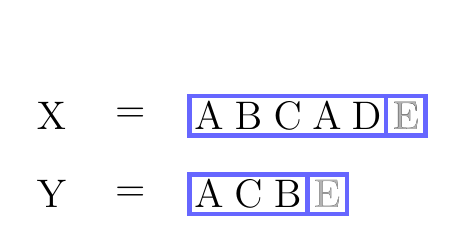
\begin{tikzpicture}

    \node at (0,3) {};
    \node at (2,2) {};

    \node[rectangle] at (-1,2) {\Large{X}};
    \node[rectangle] at (0,2) {\Large{=}};
    \node[rectangle] at (1,2) {\Large{A}};
    \node[rectangle] at (1.5,2) {\Large{B}};
    \node[rectangle] at (2,2) {\Large{C}};
    \node[rectangle] at (2.5,2) {\Large{A}};
    \node[rectangle] at (3,2) {\Large{D}};
    \onslide<1-4>{\node[rectangle] at (3.5,2) {\Large{E}};}
    \onslide<5>{\node[rectangle, text = gray!60] at (3.5,2) {\Large{E}};}
    \onslide<6->{\node[rectangle] at (3.5,2) {\Large{F}};}
    \onslide<10>{\node[rectangle, text = gray!60] at (3.5,2) {\Large{F}};}
    

    \node[rectangle] at (-1,1) {\Large{Y}};
    \node[rectangle] at (0,1) {\Large{=}};
    \node[rectangle] at (1,1) {\Large{A}};
    \node[rectangle] at (1.5,1) {\Large{C}};
    \node[rectangle] at (2,1) {\Large{B}};
    \onslide<1->{\node[rectangle] at (2.5,1) {\Large{E}};}
    \onslide<5,9>{\node[rectangle, text = gray!60] at (2.5,1) {\Large{E}};}

    
    \onslide<2,6-7>{\draw[ultra thick, blue!60] (3.5-0.25,2-0.25) rectangle (3.5+0.25,2+0.25) ;}
    \onslide<3>{\draw[ultra thick, green!80] (3.5-0.25,2-0.25) rectangle (3.5+0.25,2+0.25) ;}
    \onslide<8>{\draw[ultra thick, red!60] (3.5-0.25,2-0.25) rectangle (3.5+0.25,2+0.25) ;}

    \onslide<2,7>{\draw[ultra thick, blue!60] (2.5-0.25,1-0.25) rectangle (2.5+0.25,1+0.25) ;}
    \onslide<3>{\draw[ultra thick, green!60] (2.5-0.25,1-0.25) rectangle (2.5+0.25,1+0.25) ;}
    \onslide<8>{\draw[ultra thick, red!60] (2.5-0.25,1-0.25) rectangle (2.5+0.25,1+0.25) ;}


    \onslide<4,10>{\draw[ultra thick, blue!60] (1-0.25,2-0.25) rectangle (3+0.25,2+0.25) ;}
    \onslide<4,9>{\draw[ultra thick, blue!60] (1-0.25,1-0.25) rectangle (2+0.25,1+0.25) ;}

    \onslide<9>{\draw[ultra thick, blue!60] (1-0.25,2-0.25) rectangle (3.5+0.25,2+0.25) ;}
    \onslide<10>{\draw[ultra thick, blue!60] (1-0.25,1-0.25) rectangle (2.5+0.25,1+0.25) ;}

    

    

\end{tikzpicture}



\end{adjustbox}
\end{center}

\onslide<3->{Longest Common Subsequence : \_\_\_\_\_\_\_\_\_\_\_\_\onslide<3-5>{E}}
    
\end{frame}

 \section{Recursive Formulation}
 \begin{frame}{Recursion}
If we have two sequences

\begin{center}
    
\begin{adjustbox}{max totalsize={0.8\textwidth}{0.5\textheight}}
\begin{tikzpicture}

    \node at (0,3) {};
    \node at (2,2) {};
    \node at (2,1) {};


    \node[rectangle] at (0,2) {\Large{X}};
    \node[rectangle] at (0.5,2) {\Large{=}};
    \node[rectangle] at (1,2) {\Large{[}};
    \node[rectangle] at (1.5,2) {\Large{1}};
    \node[rectangle] at (2,2) {\Large{.}};
    \node[rectangle] at (2.5,2) {\Large{.}};
    \node[rectangle] at (3,2) {\Large{.}};
    \onslide<1,3>{\node[rectangle] at (3.5,2) {\Large{.}};}
    \onslide<2>{\node[rectangle] at (3.5,2) {\Large{a}};}
    \node[rectangle] at (4,2) {\Large{.}};
    \node[rectangle] at (4.5,2) {\Large{.}};
    \node[rectangle] at (5,2) {\Large{m}};
    \node[rectangle] at (5.5,2) {\Large{]}};

     \node[rectangle] at (7.5,2) {\Large{Y}};
    \node[rectangle] at (8,2) {\Large{=}};
    \node[rectangle] at (8.5,2) {\Large{[}};
    \node[rectangle] at (9,2) {\Large{1}};
    \node[rectangle] at (9.5,2) {\Large{.}};
    \node[rectangle] at (10,2) {\Large{.}};
    \onslide<1,3>{\node[rectangle] at (10.5,2) {\Large{.}};}
    \onslide<2>{\node[rectangle] at (10.5,2) {\Large{b}};}
    \node[rectangle] at (11,2) {\Large{.}};
    \node[rectangle] at (11.5,2) {\Large{.}};
    \node[rectangle] at (12,2) {\Large{.}};
    \node[rectangle] at (12.5,2) {\Large{n}};
    \node[rectangle] at (13,2) {\Large{]}};

    \onslide<2>\draw[very thick, red] (1.2,1.5) -- (3.8,1.5);
    \onslide<2>\draw[very thick, red] (8.8,1.5) -- (10.8,1.5);

    \onslide<3>\draw[very thick, red] (1.2,1.5) -- (5.2,1.5);
    \onslide<3>\draw[very thick, red] (8.8,1.5) -- (13.3,1.5);
   

\end{tikzpicture}
\end{adjustbox}
\end{center}

\onslide<2->{Let $LCS(a,\,b)$ denote the longest common subsequence of $x_1x_2 ... x_a$ and $y_1y_2 ... y_a$.}
\\~\
\\~\
\onslide<3->{Our goal is to find $LCS(m,\,n)$}

\end{frame}
\begin{frame}{Recursive Formulation}
\newcommand*{\xMin}{5}%
\newcommand*{\xMax}{10}%
\newcommand*{\yMin}{3}%
\newcommand*{\yMax}{11}%

\begin{tikzpicture}
    \node[rectangle] at (0,\xMin) {\large{X}};
    \node[rectangle] at (0.5,\xMin) {\large{=}};
    \node[rectangle] at (1,\xMin) {\large{[}};
    \node[rectangle] at (1.5,\xMin) {\large{1}};
    \node[rectangle] at (2,\xMin) {\large{2}};
    \node[rectangle] at (2.5,\xMin) {\large{3}};
    \node[rectangle] at (3,\xMin) {\large{.}};
    \node[rectangle] at (3.25,\xMin) {\large{.}};
    \node[rectangle] at (3.5,\xMin) {\large{.}};
    \node[rectangle] at (4,\xMin) {\large{m}};
    \node[rectangle] at (4.5,\xMin) {\large{]}};
    \onslide<2>{\draw[ultra thick, blue!60] (4-0.25,\xMin-0.25) rectangle (4+0.25,\xMin+0.25) ;}
    \onslide<2>{\draw[ultra thick, blue!60] (9.25-0.25,\xMin-0.25) rectangle (9.25+0.25,\xMin+0.25) ;}
    \onslide<3>{\draw [ultra thick, green!60] (1.25,4.75) rectangle ++(2.5,0.5);}
     \onslide<3>{\draw [ultra thick, green!60] (6.75,4.75) rectangle ++(2.25,0.5);}

    \node[rectangle] at (5.5,\xMin) {\large{Y}};
    \node[rectangle] at (6,\xMin) {\large{=}};
    \node[rectangle] at (6.5,\xMin) {\large{[}};
    \node[rectangle] at (7,\xMin) {\large{1}};
    \node[rectangle] at (7.5,\xMin) {\large{2}};
    \node[rectangle] at (8,\xMin) {\large{3}};
    \node[rectangle] at (8.25,\xMin) {\large{.}};
    \node[rectangle] at (8.5,\xMin) {\large{.}};
    \node[rectangle] at (8.75,\xMin) {\large{.}};
    \node[rectangle] at (9.25,\xMin) {\large{n}};
    \node[rectangle] at (9.75,\xMin) {\large{]}};
    \node at (0,4) {};
    
\end{tikzpicture}
    \onslide<2-3>{\large When X[m] == Y[n]}
\vspace{0.5cm}
\onslide<3>{$$ LCS(m,n) = LCS(m-1,n-1)+1 $$}
\end{frame}

\begin{frame}{Recursive Formulation}
\newcommand*{\xMin}{5}%
\newcommand*{\xMax}{10}%
\newcommand*{\yMin}{3}%
\newcommand*{\yMax}{11}%

\begin{tikzpicture}
    \node[rectangle] at (0,\xMin) {\large{X}};
    \node[rectangle] at (0.5,\xMin) {\large{=}};
    \node[rectangle] at (1,\xMin) {\large{[}};
    \node[rectangle] at (1.5,\xMin) {\large{1}};
    \node[rectangle] at (2,\xMin) {\large{2}};
    \node[rectangle] at (2.5,\xMin) {\large{3}};
    \node[rectangle] at (3,\xMin) {\large{.}};
    \node[rectangle] at (3.25,\xMin) {\large{.}};
    \node[rectangle] at (3.5,\xMin) {\large{.}};
    \node[rectangle] at (4,\xMin) {\large{m}};
    \node[rectangle] at (4.5,\xMin) {\large{]}};
    \onslide<1>{\draw[ultra thick, red!60] (4-0.25,\xMin-0.25) rectangle (4+0.25,\xMin+0.25) ;}
    \onslide<1>{\draw[ultra thick, red!60] (9.25-0.25,\xMin-0.25) rectangle (9.25+0.25,\xMin+0.25);}
    \onslide<2>{\draw [ultra thick, green!60] (1.25,4.75) rectangle ++(3,0.5);}
     \onslide<2>{\draw [ultra thick, green!60] (6.75,4.75) rectangle ++(2.25,0.5);}
     \onslide<3>{\draw [ultra thick, green!60] (1.25,4.75) rectangle ++(2.5,0.5);}
     \onslide<3>{\draw [ultra thick, green!60] (6.75,4.75) rectangle ++(2.75,0.5);}

    \node[rectangle] at (5.5,\xMin) {\large{Y}};
    \node[rectangle] at (6,\xMin) {\large{=}};
    \node[rectangle] at (6.5,\xMin) {\large{[}};
    \node[rectangle] at (7,\xMin) {\large{1}};
    \node[rectangle] at (7.5,\xMin) {\large{2}};
    \node[rectangle] at (8,\xMin) {\large{3}};
    \node[rectangle] at (8.25,\xMin) {\large{.}};
    \node[rectangle] at (8.5,\xMin) {\large{.}};
    \node[rectangle] at (8.75,\xMin) {\large{.}};
    \node[rectangle] at (9.25,\xMin) {\large{n}};
    \node[rectangle] at (9.75,\xMin) {\large{]}};
    \node at (0,4) {};
\end{tikzpicture}
    \onslide<1->{\large When X[m] != Y[n]}
\vspace{0.5cm}
\onslide<2->{$$ LCS(m,n) = max\{LCS(m,n-1),\onslide<3>{LCS(m-1,n)\} }$$}
\end{frame}

\begin{frame}{Recursive Formulation}
\newcommand*{\xMin}{5}%
\newcommand*{\xMax}{10}%
\newcommand*{\yMin}{3}%
\newcommand*{\yMax}{11}%

\begin{tikzpicture}
    \node[rectangle] at (0,\xMin) {\large{X}};
    \node[rectangle] at (0.5,\xMin) {\large{=}};
    \node[rectangle] at (1,\xMin) {\large{[}};
    \node[rectangle] at (1.5,\xMin) {\large{1}};
    \node[rectangle] at (2,\xMin) {\large{2}};
    \node[rectangle] at (2.5,\xMin) {\large{3}};
    \node[rectangle] at (3,\xMin) {\large{.}};
    \node[rectangle] at (3.25,\xMin) {\large{.}};
    \node[rectangle] at (3.5,\xMin) {\large{.}};
    \node[rectangle] at (4,\xMin) {\large{m}};
    \node[rectangle] at (4.5,\xMin) {\large{]}};


    \node[rectangle] at (5.5,\xMin) {\large{Y}};
    \node[rectangle] at (6,\xMin) {\large{=}};
    \node[rectangle] at (6.5,\xMin) {\large{[}};
    \node[rectangle] at (7,\xMin) {\large{1}};
    \node[rectangle] at (7.5,\xMin) {\large{2}};
    \node[rectangle] at (8,\xMin) {\large{3}};
    \node[rectangle] at (8.25,\xMin) {\large{.}};
    \node[rectangle] at (8.5,\xMin) {\large{.}};
    \node[rectangle] at (8.75,\xMin) {\large{.}};
    \node[rectangle] at (9.25,\xMin) {\large{n}};
    \node[rectangle] at (9.75,\xMin) {\large{]}};
    \node at (0,4) {};
\end{tikzpicture}
    \onslide<1>{\large The recursion solution:}
    \\

\small{
\[  LCS(m,n) = 
    \begin{cases} 
      LCS(m-1 , n-1)+1 & X[m] == Y[n] \\
      max\{LCS(m-1 , n),{LCS(m,n-1)\} } & X[m] != Y[n] 
   \end{cases}
\]}


\end{frame}

\begin{frame}[label=conclusion, standout]
    \begin{center}
    \LARGE What about the base case?
    \end{center}
\end{frame}

\begin{frame}{Recursive Formulation}
    \begin{center}
      \large If m == 0 then LCS(m,n) = 0\\ 
        \vspace{0.5cm}
      \large If n == 0 then LCS(m,n) = 0\\ 
    \end{center}
\end{frame}

\begin{frame}{Recursive Formulation}
    \large The final recursion solution:
       
        \small{
            \[  LCS(m,n) = 
                \begin{cases}
                  0 & m == 0 || n == 0\\
                  LCS(m-1 , n-1)+1 & X[m] == Y[n] \\
                  max\{LCS(m-1 ,n),LCS(m,n-1)\}  & X[m] != Y[n]
               \end{cases}
            \]
        }
\end{frame}



\begin{frame}[fragile]{Recursion}
\scriptsize{
$
    LCS(m,n)=\begin{cases}
    0 \quad & \text{if }\; m = 0  \quad or \quad  n = 0 \\
    LCS(m-1, n-1) + 1  \quad & \text{if }\; X[m] = Y[n] \\
    MAX(LCS(m-1,n), LCS(m,n-1)) \quad &\text{if }\; X[m] != Y[n]  \\ 
     \end{cases}
$
}
\\~\
\\~\
\small{

%\onslide<1> { \begin{tcolorbox}[colback=black!5,colframe=cyan!50!blue] } 
    \begin{minted}{python}
    def LCS(X[1..m], Y[1..n]) :
        if m = 0 or n = 0
            return 0
    \end{minted}
%\onslide<1> { \end{tcolorbox} } 
    \pause
 %\onslide<2> {     \begin{tcolorbox}[colback=black!5,colframe=green!60!blue] } 
    \begin{minted}{python}
        if X[m] = Y[n] :
            result = LCS(m-1, n-1) + 1
    \end{minted}
%\onslide<2> {\end{tcolorbox}}
    \pause
%\onslide<3> {   \begin{tcolorbox}[colback=black!5,colframe=pink!60!blue] }
    \begin{minted}{python}
        else :
            result = max(LCS(m-1, n), LCS(m, n-1))
    \end{minted}
    \pause
    \begin{minted}{python}
        return result
    \end{minted}
%\onslide<3> {\end{tcolorbox} }
}

\end{frame}



\begin{frame}{Frame Title}

\begin{center}
    

\tikzset{font=\fontsize{10}{10}\selectfont}
\begin{adjustbox}{max totalsize={\textwidth}{0.9\textheight}}
\begin{tikzpicture}[level distance=2cm,
  level 1/.style={sibling distance=8cm},
  level 2/.style={sibling distance=5cm},
  level 3/.style={sibling distance=2.5cm}]
  \node {LCS(m,n)}
     child {
      node {LCS(m-1 , n)}
      child {
        node(a0) {LCS(m-2 , n)}       
      }
      child {
        node(a1) {LCS(m-1 , n-1)}
      }
    }
     child {
      node {LCS(m , n-1)}
      child {
        node(a2) {LCS(m-1 , n-1)}
      }
      child {
        node(a3) {LCS(m-1 , n-2)}
      }
    };
\draw[ultra thick , dotted] (a0) -- +(-90:2cm);
\draw[ultra thick , dotted] (a1) -- +(-90:2cm);
\draw[ultra thick , dotted] (a2) -- +(-90:2cm);
\draw[ultra thick , dotted] (a3) -- +(-90:2cm);
\end{tikzpicture}
\end{adjustbox}
\\~\
\\~\
\onslide <2> 
{
   \textcolor{blue!80}{So the time complexity is $O(2^n)$} 
}


\end{center}
\end{frame}




\begin{frame}[fragile]{Memoized Algorithm}

\scriptsize{
   $
    LCS(m,n)=\begin{cases}
          0 \quad & \text{if }\; m = 0  \quad or \quad  n = 0 \\
           LCS(m-1, n-1) + 1  \quad & \text{if }\; X[m] = Y[n] \\
          MAX(LCS(m-1,n), LCS(m,n-1)) \quad &\text{if }\; X[m] != Y[n]  \\
     \end{cases}
$
}
\\~\
\\~\

\begin{multicols}{2}
\small{
    \begin{minted}{python}
    def LCS(X[1..m], Y[1..n]) :
        if m = 0 or n = 0
            return 0
        if LCS_memo[m][n] != -INF:
            return LCS_memo[m][n]
        else if X[m] = Y[n] :
            result = LCS(m-1, n-1) + 1
        else :
            result = max(LCS(m-1, n), LCS(m, n-1))
        LCS_memo[m][n] = result
        return result
    \end{minted}}
    
\columnbreak
\pause 
\begin{tcolorbox}[colback=green!5,colframe=green!40!black]
     \textcolor{black!80}{ Time complexity is $O(mn)$} 
\end{tcolorbox}
\end{multicols}
\end{frame}



\section{Using Dynamic Programming}
\begin{frame}{Dynamic Programming}

\newcommand*{\xMin}{3}%
\newcommand*{\xMax}{10}%
\newcommand*{\yMin}{3}%
\newcommand*{\yMax}{11}%



\begin{columns}


\column{0.7\textwidth}
    \begin{center}


\begin{adjustbox}{max totalsize={0.95\textwidth}{0.8\textheight}}
\begin{tikzpicture}

    \foreach \i in {\xMin,...,\xMax} {
        \draw [very thin,brown] (\i,\yMin) -- (\i,\yMax);
    }
    \foreach \i in {\yMin,...,\yMax} {
        \draw [very thin,brown] (\xMin,\i) -- (\xMax,\i);
    }

    
    \foreach \i in {0,...,6} {
        \node at (3 + \i + 0.5, \yMax + 1.5) {\Large $\i$};
        \node at (3+\i + 0.6, \yMax - 0.6) {{\onslide<2->{\Large $0$}}};
    }

    \foreach \i in {0,...,7} {
        \node at (\xMin - 1.5, 3 + 7 - \i + 0.5) {\Large $\i$};
        \node at (\xMin + 0.6, 4+\i - 0.6) {{\onslide<2->{\Large $0$}}};
    }

    % row selection
    \onslide<3-14>{\draw[dp_select_circle] (\xMin - 0.5, 3 + 7 - 1 + 0.5) circle (0.35);}
    \onslide<19-20>{\draw[dp_select_circle] (\xMin - 0.5, 3 + 7 - 2 + 0.5) circle (0.35);}
    % \onslide<2>{\draw[dp_select_circle] (\xMin - 0.5, 3 + 7 - 3 + 0.5) circle (0.35);}
    % \onslide<2>{\draw[dp_select_circle] (\xMin - 0.5, 3 + 7 - 4 + 0.5) circle (0.35);}
    % \onslide<2>{\draw[dp_select_circle] (\xMin - 0.5, 3 + 7 - 5+ 0.5) circle (0.35);}
    % \onslide<2>{\draw[dp_select_circle] (\xMin - 0.5, 3 + 7 - 6 + 0.5) circle (0.35);}
    % \onslide<2>{\draw[dp_select_circle] (\xMin - 0.5, 3 + 7 - 7 + 0.5) circle (0.35);}

    % row match
    \onslide<9-10,13-14>{\draw[dp_match_circle] (\xMin - 0.5, 3 + 7 - 1 + 0.5) circle (0.35);}
    \onslide<15-18>{\draw[dp_match_circle] (\xMin - 0.5, 3 + 7 - 2 + 0.5) circle (0.35);}
    % \onslide<2>{\draw[dp_match_circle] (\xMin - 0.5, 3 + 7 - 3 + 0.5) circle (0.35);}
    % \onslide<2>{\draw[dp_match_circle] (\xMin - 0.5, 3 + 7 - 4 + 0.5) circle (0.35);}
    % \onslide<2>{\draw[dp_match_circle] (\xMin - 0.5, 3 + 7 - 5+ 0.5) circle (0.35);}
    % \onslide<2>{\draw[dp_match_circle] (\xMin - 0.5, 3 + 7 - 6 + 0.5) circle (0.35);}
    % \onslide<2>{\draw[dp_match_circle] (\xMin - 0.5, 3 + 7 - 7 + 0.5) circle (0.35);}


    %column select
    \onslide<3-4>{\draw[dp_select_circle] (3 + 1 + 0.5, \yMax + 0.5) circle (0.35);}
    \onslide<5-6>{\draw[dp_select_circle] (3 + 2 + 0.5, \yMax + 0.5) circle (0.35);}
    \onslide<7-8>{\draw[dp_select_circle] (3 + 3 + 0.5, \yMax + 0.5) circle (0.35);}
    %\onslide<2>{\draw[dp_select_circle] (3 + 4 + 0.5, \yMax + 0.5) circle (0.35);}
    \onslide<11-12>{\draw[dp_select_circle] (3 + 5 + 0.5, \yMax + 0.5) circle (0.35);}
    \onslide<19,20>{\draw[dp_select_circle] (3 + 6 + 0.5, \yMax + 0.5) circle (0.35);}

    %column match
    \onslide<15-16>{\draw[dp_match_circle] (3 + 1 + 0.5, \yMax + 0.5) circle (0.35);}
    %\onslide<2>{\draw[dp_match_circle] (3 + 2 + 0.5, \yMax + 0.5) circle (0.35);}
    %\onslide<2>{\draw[dp_match_circle] (3 + 3 + 0.5, \yMax + 0.5) circle (0.35);}
    \onslide<9-10>{\draw[dp_match_circle] (3 + 4 + 0.5, \yMax + 0.5) circle (0.35);}
    \onslide<17-18>{\draw[dp_match_circle] (3 + 5 + 0.5, \yMax + 0.5) circle (0.35);}
    \onslide<13-14>{\draw[dp_match_circle] (3 + 6 + 0.5, \yMax + 0.5) circle (0.35);}

    

    \node at (3 + 0 + 0.5, \yMax + 0.5) {\Large $y_j$};
    \node at (3 + 1 + 0.5, \yMax + 0.5) {\Large $B$};
    \node at (3 + 2 + 0.5, \yMax + 0.5) {\Large $D$};
    \node at (3 + 3 + 0.5, \yMax + 0.5) {\Large $C$};
    \node at (3 + 4 + 0.5, \yMax + 0.5) {\Large $A$};
    \node at (3 + 5 + 0.5, \yMax + 0.5) {\Large $B$};
    \node at (3 + 6 + 0.5, \yMax + 0.5) {\Large $A$};

    \node at (\xMin - 0.5, 3 + 7 - 0 + 0.5) {\Large $x_i$};
    \node at (\xMin - 0.5, 3 + 7 - 1 + 0.5) {\Large $A$};
    \node at (\xMin - 0.5, 3 + 7 - 2 + 0.5) {\Large $B$};
    \node at (\xMin - 0.5, 3 + 7 - 3 + 0.5) {\Large $C$};
    \node at (\xMin - 0.5, 3 + 7 - 4 + 0.5) {\Large $B$};
    \node at (\xMin - 0.5, 3 + 7 - 5 + 0.5) {\Large $D$};
    \node at (\xMin - 0.5, 3 + 7 - 6 + 0.5) {\Large $A$};
    \node at (\xMin - 0.5, 3 + 7 - 7 + 0.5) {\Large $B$};
    

    % row 1
    \node at (\xMin + 0.6 + 1, 4 - 0.6 + 6) {{\onslide<4->{\Large $0$}}}; %11
    \onslide<4->{\draw[dp_table_arrow] (\xMin + 0.2 + 1, 4 - 0.3 + 6) -- (\xMin + 0.2 + 1, 4 - 0.5 + 7);} % vertical
    
    \node at (\xMin + 0.6 + 2, 4 - 0.6 + 6) {{\onslide<6->{\Large $0$}}}; %12
    \onslide<6->{\draw[dp_table_arrow] (\xMin + 0.2 + 2, 4 - 0.3 + 6) -- (\xMin + 0.2 + 2, 4 - 0.5 + 7);}
    
    \node at (\xMin + 0.6 + 3, 4 - 0.6 + 6) {{\onslide<8->{\Large $0$}}}; %13
    \onslide<8->{\draw[dp_table_arrow] (\xMin + 0.2 + 3, 4 - 0.3 + 6) -- (\xMin + 0.2 + 3, 4 - 0.5 + 7);}
    
    \node at (\xMin + 0.6 + 4, 4 - 0.6 + 6) {{\onslide<10->{\Large $1$}}}; %14
    \onslide<10->{\draw[dp_table_arrow] (\xMin + 0.3 + 4, 4 - 0.4 + 6) -- (\xMin - 0.2 + 4, 4 - 0.6 + 7);} % angle
    
    \node at (\xMin + 0.6 + 5, 4 - 0.6 + 6) {{\onslide<11->{\Large $1$}}}; %15
    \onslide<11->{\draw[dp_table_arrow] (\xMin + 0.3 + 5, 4 - 0.3 + 6) -- (\xMin - 0.3 + 5, 4 - 0.3 + 6);} % horizontal
    
    \node at (\xMin + 0.6 + 6, 4 - 0.6 + 6) {{\onslide<13->{\Large $1$}}}; %16
    \onslide<13->{\draw[dp_table_arrow] (\xMin + 0.3 + 6, 4 - 0.4 + 6) -- (\xMin - 0.2 + 6, 4 - 0.6 + 7);} % angle




    % row 2
    \node at (\xMin + 0.6 + 1, 4 - 0.6 + 5) {{\onslide<15->{\Large $1$}}}; %21
    \onslide<15->{\draw[dp_table_arrow] (\xMin + 0.3 + 1, 4 - 0.4 + 5) -- (\xMin - 0.2 + 1, 4 - 0.6 + 6);} % angle
    
    \node at (\xMin + 0.6 + 2, 4 - 0.6 + 5) {{\onslide<17->{\Large $1$}}}; %22
    \onslide<17->{\draw[dp_table_arrow] (\xMin + 0.3 + 2, 4 - 0.3 + 5) -- (\xMin - 0.3 + 2, 4 - 0.3 + 5);} % horizontal
    
    \node at (\xMin + 0.6 + 3, 4 - 0.6 + 5) {{\onslide<17->{\Large $1$}}}; %23
    \onslide<17->{\draw[dp_table_arrow] (\xMin + 0.3 + 3, 4 - 0.3 + 5) -- (\xMin - 0.3 + 3, 4 - 0.3 + 5);} % horizontal
    
    \node at (\xMin + 0.6 + 4, 4 - 0.6 + 5) {{\onslide<17->{\Large $1$}}}; %24
    \onslide<17->{\draw[dp_table_arrow] (\xMin + 0.2 + 4, 4 - 0.3 + 5) -- (\xMin + 0.2 + 4, 4 - 0.5 + 6);} % vertical
    
    \node at (\xMin + 0.6 + 5, 4 - 0.6 + 5) {{\onslide<17->{\Large $2$}}}; %25
    \onslide<17->{\draw[dp_table_arrow] (\xMin + 0.3 + 5, 4 - 0.4 + 5) -- (\xMin - 0.2 + 5, 4 - 0.6 + 6);} % angle
    
    \node at (\xMin + 0.6 + 6, 4 - 0.6 + 5) {{\onslide<20->{\Large $2$}}}; %26
    \onslide<20->{\draw[dp_table_arrow] (\xMin + 0.3 + 6, 4 - 0.3 + 5) -- (\xMin - 0.3 + 6, 4 - 0.3 + 5);} % horizontal



    % row 3
    \node at (\xMin + 0.6 + 1, 4 - 0.6 + 4) {{\onslide<21->{\Large $1$}}}; %31
    \onslide<21->{\draw[dp_table_arrow] (\xMin + 0.2 + 1, 4 - 0.3 + 4) -- (\xMin + 0.2 + 1, 4 - 0.5 + 5);} % vertical
    
    \node at (\xMin + 0.6 + 2, 4 - 0.6 + 4) {{\onslide<21->{\Large $1$}}}; %32
    \onslide<21->{\draw[dp_table_arrow] (\xMin + 0.2 + 2, 4 - 0.3 + 4) -- (\xMin + 0.2 + 2, 4 - 0.5 + 5);} % vertical
    
    \node at (\xMin + 0.6 + 3, 4 - 0.6 + 4) {{\onslide<22->{\Large $2$}}}; %33
    \onslide<22->{\draw[dp_table_arrow] (\xMin + 0.3 + 3, 4 - 0.4 + 4) -- (\xMin - 0.2 + 3, 4 - 0.6 + 5);} % angle
    
    \node at (\xMin + 0.6 + 4, 4 - 0.6 + 4) {{\onslide<22->{\Large $2$}}}; %34
    \onslide<22->{\draw[dp_table_arrow] (\xMin + 0.3 + 4, 4 - 0.3 + 4) -- (\xMin - 0.3 + 4, 4 - 0.3 + 4);} % horizontal
    
    \node at (\xMin + 0.6 + 5, 4 - 0.6 + 4) {{\onslide<22->{\Large $2$}}}; %35
    \onslide<22->{\draw[dp_table_arrow] (\xMin + 0.2 + 5, 4 - 0.3 + 4) -- (\xMin + 0.2 + 5, 4 - 0.5 + 5);} % vertical
    
    \node at (\xMin + 0.6 + 6, 4 - 0.6 + 4) {{\onslide<22->{\Large $2$}}}; %36
    \onslide<22->{\draw[dp_table_arrow] (\xMin + 0.2 + 6, 4 - 0.3 + 4) -- (\xMin + 0.2 + 6, 4 - 0.5 + 5);} % vertical



    % row 4
    \node at (\xMin + 0.6 + 1, 4 - 0.6 + 3) {{\onslide<23->{\Large $1$}}}; %41
    \onslide<23->{\draw[dp_table_arrow] (\xMin + 0.3 + 1, 4 - 0.4 + 3) -- (\xMin - 0.2 + 1, 4 - 0.6 + 4);} % angle
    \node at (\xMin + 0.6 + 2, 4 - 0.6 + 3) {{\onslide<23->{\Large $1$}}}; %42
    \onslide<23->{\draw[dp_table_arrow] (\xMin + 0.2 + 2, 4 - 0.3 + 3) -- (\xMin + 0.2 + 2, 4 - 0.5 + 4);} % vertical

    \node at (\xMin + 0.6 + 3, 4 - 0.6 + 3) {{\onslide<23->{\Large $2$}}}; %43
    \onslide<23->{\draw[dp_table_arrow] (\xMin + 0.2 + 3, 4 - 0.3 + 3) -- (\xMin + 0.2 + 3, 4 - 0.5 + 4);} % vertical

    \node at (\xMin + 0.6 + 4, 4 - 0.6 + 3) {{\onslide<23->{\Large $2$}}}; %44
    \onslide<23->{\draw[dp_table_arrow] (\xMin + 0.2 + 4, 4 - 0.3 + 3) -- (\xMin + 0.2 + 4, 4 - 0.5 + 4);} % vertical

    \node at (\xMin + 0.6 + 5, 4 - 0.6 + 3) {{\onslide<23->{\Large $3$}}}; %45
    \onslide<23->{\draw[dp_table_arrow] (\xMin + 0.3 + 5, 4 - 0.4 + 3) -- (\xMin - 0.2 + 5, 4 - 0.6 + 4);} % angle
    
    \node at (\xMin + 0.6 + 6, 4 - 0.6 + 3) {{\onslide<23->{\Large $3$}}}; %46
    \onslide<23->{\draw[dp_table_arrow] (\xMin + 0.3 + 6, 4 - 0.3 + 3) -- (\xMin - 0.3 + 6, 4 - 0.3 + 3);} % horizontal
    

     % row 5
    \node at (\xMin + 0.6 + 1, 4 - 0.6 + 2) {{\onslide<24->{\Large $1$}}}; %51
    \onslide<24->{\draw[dp_table_arrow] (\xMin + 0.2 + 1, 4 - 0.3 + 2) -- (\xMin + 0.2 + 1, 4 - 0.5 + 3);} % vertical
    \node at (\xMin + 0.6 + 2, 4 - 0.6 + 2) {{\onslide<24->{\Large $2$}}}; %52
    \onslide<24->{\draw[dp_table_arrow] (\xMin + 0.3 + 2, 4 - 0.4 + 2) -- (\xMin - 0.2 + 2, 4 - 0.6 + 3);} % angle
    \node at (\xMin + 0.6 + 3, 4 - 0.6 + 2) {{\onslide<24->{\Large $2$}}}; %53
     \onslide<24->{\draw[dp_table_arrow] (\xMin + 0.2 + 3, 4 - 0.3 + 2) -- (\xMin + 0.2 + 3, 4 - 0.5 + 3);} % vertical
    \node at (\xMin + 0.6 + 4, 4 - 0.6 + 2) {{\onslide<24->{\Large $2$}}}; %54
     \onslide<24->{\draw[dp_table_arrow] (\xMin + 0.2 + 4, 4 - 0.3 + 2) -- (\xMin + 0.2 + 4, 4 - 0.5 + 3);} % vertical
    \node at (\xMin + 0.6 + 5, 4 - 0.6 + 2) {{\onslide<24->{\Large $3$}}}; %55
     \onslide<24->{\draw[dp_table_arrow] (\xMin + 0.2 + 5, 4 - 0.3 + 2) -- (\xMin + 0.2 + 5, 4 - 0.5 + 3);} % vertical
    \node at (\xMin + 0.6 + 6, 4 - 0.6 + 2) {{\onslide<24->{\Large $3$}}}; %56
     \onslide<24->{\draw[dp_table_arrow] (\xMin + 0.2 + 6, 4 - 0.3 + 2) -- (\xMin + 0.2 + 6, 4 - 0.5 + 3);} % vertical

    % row 6
    \node at (\xMin + 0.6 + 1, 4 - 0.6 + 1) {{\onslide<25->{\Large $1$}}}; %61
    \onslide<25->{\draw[dp_table_arrow] (\xMin + 0.2 + 1, 4 - 0.3 + 1) -- (\xMin + 0.2 + 1, 4 - 0.5 + 2);} % vertical
    \node at (\xMin + 0.6 + 2, 4 - 0.6 + 1) {{\onslide<25->{\Large $2$}}}; %62
    \onslide<25->{\draw[dp_table_arrow] (\xMin + 0.2 + 2, 4 - 0.3 + 1) -- (\xMin + 0.2 + 2, 4 - 0.5 + 2);} % vertical
    \node at (\xMin + 0.6 + 3, 4 - 0.6 + 1) {{\onslide<25->{\Large $2$}}}; %63
    \onslide<25->{\draw[dp_table_arrow] (\xMin + 0.2 + 3, 4 - 0.3 + 1) -- (\xMin + 0.2 + 3, 4 - 0.5 + 2);} % vertical
    \node at (\xMin + 0.6 + 4, 4 - 0.6 + 1) {{\onslide<25->{\Large $3$}}}; %64
    \onslide<25->{\draw[dp_table_arrow] (\xMin + 0.3 + 4, 4 - 0.4 + 1) -- (\xMin - 0.2 + 4, 4 - 0.6 + 2);} % angle
    \node at (\xMin + 0.6 + 5, 4 - 0.6 + 1) {{\onslide<25->{\Large $3$}}}; %65
    \onslide<25->{\draw[dp_table_arrow] (\xMin + 0.2 + 5, 4 - 0.3 + 1) -- (\xMin + 0.2 + 5, 4 - 0.5 + 2);} % vertical
    \node at (\xMin + 0.6 + 6, 4 - 0.6 + 1) {{\onslide<25->{\Large $4$}}}; %66
    \onslide<25->{\draw[dp_table_arrow] (\xMin + 0.3 + 6, 4 - 0.4 + 1) -- (\xMin - 0.2 + 6, 4 - 0.6 + 2);} % angle

    % row 7
    \node at (\xMin + 0.6 + 1, 4 - 0.6 + 0) {{\onslide<26->{\Large $1$}}}; %71
    \onslide<26->{\draw[dp_table_arrow] (\xMin + 0.3 + 1, 4 - 0.4 + 0) -- (\xMin - 0.2 + 1, 4 - 0.6 + 1);} % angle
    \node at (\xMin + 0.6 + 2, 4 - 0.6 + 0) {{\onslide<26->{\Large $2$}}}; %72
    \onslide<26->{\draw[dp_table_arrow] (\xMin + 0.2 + 2, 4 - 0.3 + 0) -- (\xMin + 0.2 + 2, 4 - 0.5 + 1);} % vertical
    \node at (\xMin + 0.6 + 3, 4 - 0.6 + 0) {{\onslide<26->{\Large $2$}}}; %73
    \onslide<26->{\draw[dp_table_arrow] (\xMin + 0.2 + 3, 4 - 0.3 + 0) -- (\xMin + 0.2 + 3, 4 - 0.5 + 1);} % vertical
    \node at (\xMin + 0.6 + 4, 4 - 0.6 + 0) {{\onslide<26->{\Large $3$}}}; %74
    \onslide<26->{\draw[dp_table_arrow] (\xMin + 0.2 + 4, 4 - 0.3 + 0) -- (\xMin + 0.2 + 4, 4 - 0.5 + 1);} % vertical
    \node at (\xMin + 0.6 + 5, 4 - 0.6 + 0) {{\onslide<26->{\Large $4$}}}; %75
    \onslide<26->{\draw[dp_table_arrow] (\xMin + 0.3 + 5, 4 - 0.4 + 0) -- (\xMin - 0.2 + 5, 4 - 0.6 + 1);} % angle
    \node at (\xMin + 0.6 + 6, 4 - 0.6 + 0) {{\onslide<26->{\Large $4$}}}; %76
    \onslide<26->{\draw[dp_table_arrow] (\xMin + 0.2 + 6, 4 - 0.3 + 0) -- (\xMin + 0.2 + 6, 4 - 0.5 + 1);} % vertical
    
    \onslide<27>{\draw[thick, red] (\xMin + 6.5, 3.5) circle (0.8); }


\end{tikzpicture}
\end{adjustbox}
\end{center}

\column{0.5\textwidth}
{\fontsize{6pt}{6pt}\selectfont
If m=0 or n=0\\
\qquad LCS(m,n) = 0\\~\ \\~\ Else if X[m] = Y[n]\\
\qquad LCS(m,n) = LCS(m-1, n-1) + 1\\~\ \\~\ Else\\
\qquad LCS(m,n) = max( LCS(m-1,n), LCS(m, n-1))
}


\end{columns}
\end{frame}

\input{DP5}
\begin{frame}[label=conclusion, standout]
    \begin{center}
    \LARGE What if we want to find the subsequence too?
    \end{center}
\end{frame}


\begin{frame}{Going back}

\newcommand*{\xMin}{3}%
\newcommand*{\xMax}{10}%
\newcommand*{\yMin}{3}%
\newcommand*{\yMax}{11}%



\begin{columns}


\column{0.7\textwidth}
    \begin{center}


\begin{adjustbox}{max totalsize={0.95\textwidth}{0.8\textheight}}
\begin{tikzpicture}


    % eikhane rectangle 
    \onslide<2-> { \draw[dp_no_match_rect] (\xMin + 6, 3) rectangle (\xMin+1+6, 4); 
   \draw[dp_select_circle] (\xMin - 0.5, 3 + 7 - 7 + 0.5) circle (0.35);
   \draw[dp_select_circle] (3 + 6 + 0.5, \yMax + 0.5) circle (0.35);}
   
    \onslide<3-> { \draw[dp_match_rect] (\xMin + 6, 4) rectangle (\xMin+1+6, 5);
   \draw[dp_match_circle] (\xMin - 0.5, 3 + 7 - 6 + 0.5) circle (0.35); 
   \draw[dp_match_circle] (3 + 6 + 0.5, \yMax + 0.5) circle (0.35);}
    
    \onslide<4-> { \draw[dp_no_match_rect] (\xMin + 5, 5) rectangle (\xMin+1+5, 6);
    \draw[dp_select_circle] (\xMin - 0.5, 3 + 7 - 5+ 0.5) circle (0.35);
    \draw[dp_select_circle] (3 + 5 + 0.5, \yMax + 0.5) circle (0.35);}
    
    \onslide<5-> { \draw[dp_match_rect] (\xMin + 5, 6) rectangle (\xMin+1+5, 7); 
    \draw[dp_match_circle] (\xMin - 0.5, 3 + 7 - 4 + 0.5) circle (0.35);
    \draw[dp_match_circle] (3 + 5 + 0.5, \yMax + 0.5) circle (0.35);}

    
     \onslide<6-> { \draw[dp_no_match_rect] (\xMin + 4, 7) rectangle (\xMin+1+4, 8);
    \draw[dp_select_circle] (\xMin - 0.5, 3 + 7 - 3 + 0.5) circle (0.35);
   \draw[dp_select_circle] (3 + 4 + 0.5, \yMax + 0.5) circle (0.35); }
     
    \onslide<7-> { \draw[dp_match_rect] (\xMin + 3, 7) rectangle (\xMin+1+3, 8); 
    \draw[dp_match_circle] (\xMin - 0.5, 3 + 7 - 3 + 0.5) circle (0.35);
    \draw[dp_match_circle] (3 + 3 + 0.5, \yMax + 0.5) circle (0.35);
    }
    
    \onslide<8-> { \draw[dp_no_match_rect] (\xMin + 2, 8) rectangle (\xMin+1+2, 9);
    \draw[dp_select_circle] (\xMin - 0.5, 3 + 7 - 2 + 0.5) circle (0.35);
    \draw[dp_select_circle] (3 + 2 + 0.5, \yMax + 0.5) circle (0.35);}
    
    \onslide<9-> { \draw[dp_match_rect] (\xMin + 1, 8) rectangle (\xMin+1+1, 9);
   \draw[dp_match_circle] (\xMin - 0.5, 3 + 7 - 2 + 0.5) circle (0.35); 
   \draw[dp_match_circle] (3 + 1 + 0.5, \yMax + 0.5) circle (0.35);}
    
     \onslide<10-> { \draw[dp_no_match_rect] (\xMin , 9) rectangle (\xMin+1, 10);
     \draw[dp_select_circle] (\xMin - 0.5, 3 + 7 - 1 + 0.5) circle (0.35);
     
     }
    
    
    \foreach \i in {\xMin,...,\xMax} {
        \draw [very thin,brown] (\i,\yMin) -- (\i,\yMax);
    }
    \foreach \i in {\yMin,...,\yMax} {
        \draw [very thin,brown] (\xMin,\i) -- (\xMax,\i);
    }

    
    \foreach \i in {0,...,6} {
        \node at (3 + \i + 0.5, \yMax + 1.5) {\Large $\i$};
        \node at (3+\i + 0.6, \yMax - 0.6) {\Large $0$};
    }

    \foreach \i in {0,...,7} {
        \node at (\xMin - 1.5, 3 + 7 - \i + 0.5) {\Large $\i$};
        \node at (\xMin + 0.6, 4+\i - 0.6) {\Large $0$};
    }



    

    \node at (3 + 0 + 0.5, \yMax + 0.5) {\Large $y_j$};
    \node at (3 + 1 + 0.5, \yMax + 0.5) {\Large $B$};
    \node at (3 + 2 + 0.5, \yMax + 0.5) {\Large $D$};
    \node at (3 + 3 + 0.5, \yMax + 0.5) {\Large $C$};
    \node at (3 + 4 + 0.5, \yMax + 0.5) {\Large $A$};
    \node at (3 + 5 + 0.5, \yMax + 0.5) {\Large $B$};
    \node at (3 + 6 + 0.5, \yMax + 0.5) {\Large $A$};

    \node at (\xMin - 0.5, 3 + 7 - 0 + 0.5) {\Large $x_i$};
    \node at (\xMin - 0.5, 3 + 7 - 1 + 0.5) {\Large $A$};
    \node at (\xMin - 0.5, 3 + 7 - 2 + 0.5) {\Large $B$};
    \node at (\xMin - 0.5, 3 + 7 - 3 + 0.5) {\Large $C$};
    \node at (\xMin - 0.5, 3 + 7 - 4 + 0.5) {\Large $B$};
    \node at (\xMin - 0.5, 3 + 7 - 5 + 0.5) {\Large $D$};
    \node at (\xMin - 0.5, 3 + 7 - 6 + 0.5) {\Large $A$};
    \node at (\xMin - 0.5, 3 + 7 - 7 + 0.5) {\Large $B$};
    

    % row 1
    \node at (\xMin + 0.6 + 1, 4 - 0.6 + 6) {\Large $0$}; %11
    \draw[dp_table_arrow] (\xMin + 0.2 + 1, 4 - 0.3 + 6) -- (\xMin + 0.2 + 1, 4 - 0.5 + 7);
    
    \node at (\xMin + 0.6 + 2, 4 - 0.6 + 6) {\Large $0$}; %12
    \draw[dp_table_arrow] (\xMin + 0.2 + 2, 4 - 0.3 + 6) -- (\xMin + 0.2 + 2, 4 - 0.5 + 7);
    
    
    \node at (\xMin + 0.6 + 3, 4 - 0.6 + 6) {\Large $0$}; %13
    \draw[dp_table_arrow] (\xMin + 0.2 + 3, 4 - 0.3 + 6) -- (\xMin + 0.2 + 3, 4 - 0.5 + 7);
    
    \node at (\xMin + 0.6 + 4, 4 - 0.6 + 6) {\Large $1$}; %14
    \draw[dp_table_arrow] (\xMin + 0.3 + 4, 4 - 0.4 + 6) -- (\xMin - 0.2 + 4, 4 - 0.6 + 7);
    
    \node at (\xMin + 0.6 + 5, 4 - 0.6 + 6) {\Large $1$}; %15
    \draw[dp_table_arrow] (\xMin + 0.3 + 5, 4 - 0.3 + 6) -- (\xMin - 0.3 + 5, 4 - 0.3 + 6);
    
    \node at (\xMin + 0.6 + 6, 4 - 0.6 + 6) {\Large $1$}; %16
    \draw[dp_table_arrow] (\xMin + 0.3 + 6, 4 - 0.4 + 6) -- (\xMin - 0.2 + 6, 4 - 0.6 + 7);




    % row 2
    \node at (\xMin + 0.6 + 1, 4 - 0.6 + 5) {\Large $1$}; %21
    \draw[dp_table_arrow] (\xMin + 0.3 + 1, 4 - 0.4 + 5) -- (\xMin - 0.2 + 1, 4 - 0.6 + 6);
    
    \node at (\xMin + 0.6 + 2, 4 - 0.6 + 5) {\Large $1$}; %22
    \draw[dp_table_arrow] (\xMin + 0.3 + 2, 4 - 0.3 + 5) -- (\xMin - 0.3 + 2, 4 - 0.3 + 5);
    
    \node at (\xMin + 0.6 + 3, 4 - 0.6 + 5) {\Large $1$}; %23
    \draw[dp_table_arrow] (\xMin + 0.3 + 3, 4 - 0.3 + 5) -- (\xMin - 0.3 + 3, 4 - 0.3 + 5);
    
    \node at (\xMin + 0.6 + 4, 4 - 0.6 + 5) {\Large $1$}; %24
    \draw[dp_table_arrow] (\xMin + 0.2 + 4, 4 - 0.3 + 5) -- (\xMin + 0.2 + 4, 4 - 0.5 + 6);
    
    \node at (\xMin + 0.6 + 5, 4 - 0.6 + 5) {\Large $2$}; %25
    \node at (\xMin + 0.6 + 6, 4 - 0.6 + 5) {\Large $2$}; %26
    \draw[dp_table_arrow] (\xMin + 0.3 + 6, 4 - 0.3 + 5) -- (\xMin - 0.3 + 6, 4 - 0.3 + 5);



    % row 3
    \node at (\xMin + 0.6 + 1, 4 - 0.6 + 4) {\Large $1$}; %31
    \draw[dp_table_arrow] (\xMin + 0.2 + 1, 4 - 0.3 + 4) -- (\xMin + 0.2 + 1, 4 - 0.5 + 5);
    
    \node at (\xMin + 0.6 + 2, 4 - 0.6 + 4) {\Large $1$}; %32
    \draw[dp_table_arrow] (\xMin + 0.2 + 2, 4 - 0.3 + 4) -- (\xMin + 0.2 + 2, 4 - 0.5 + 5);
    
    \node at (\xMin + 0.6 + 3, 4 - 0.6 + 4) {\Large $2$}; %33
    \draw[dp_table_arrow] (\xMin + 0.3 + 3, 4 - 0.4 + 4) -- (\xMin - 0.2 + 3, 4 - 0.6 + 5);
    
    \node at (\xMin + 0.6 + 4, 4 - 0.6 + 4) {\Large $2$}; %34
    \draw[dp_table_arrow] (\xMin + 0.3 + 4, 4 - 0.3 + 4) -- (\xMin - 0.3 + 4, 4 - 0.3 + 4);
    
    \node at (\xMin + 0.6 + 5, 4 - 0.6 + 4) {\Large $2$}; %35
    \draw[dp_table_arrow] (\xMin + 0.2 + 5, 4 - 0.3 + 4) -- (\xMin + 0.2 + 5, 4 - 0.5 + 5);
    
    \node at (\xMin + 0.6 + 6, 4 - 0.6 + 4) {\Large $2$}; %36
    \draw[dp_table_arrow] (\xMin + 0.2 + 6, 4 - 0.3 + 4) -- (\xMin + 0.2 + 6, 4 - 0.5 + 5);



    % row 4
    \node at (\xMin + 0.6 + 1, 4 - 0.6 + 3) {\Large $1$}; %41
    \draw[dp_table_arrow] (\xMin + 0.3 + 1, 4 - 0.4 + 3) -- (\xMin - 0.2 + 1, 4 - 0.6 + 4);
    \node at (\xMin + 0.6 + 2, 4 - 0.6 + 3) {\Large $1$}; %42
    \draw[dp_table_arrow] (\xMin + 0.2 + 2, 4 - 0.3 + 3) -- (\xMin + 0.2 + 2, 4 - 0.5 + 4);

    \node at (\xMin + 0.6 + 3, 4 - 0.6 + 3) {\Large $2$}; %43
    \draw[dp_table_arrow] (\xMin + 0.2 + 3, 4 - 0.3 + 3) -- (\xMin + 0.2 + 3, 4 - 0.5 + 4);

    \node at (\xMin + 0.6 + 4, 4 - 0.6 + 3) {\Large $2$}; %44
    \draw[dp_table_arrow] (\xMin + 0.2 + 4, 4 - 0.3 + 3) -- (\xMin + 0.2 + 4, 4 - 0.5 + 4);

    \node at (\xMin + 0.6 + 5, 4 - 0.6 + 3) {\Large $3$}; %45
    \draw[dp_table_arrow] (\xMin + 0.3 + 5, 4 - 0.4 + 3) -- (\xMin - 0.2 + 5, 4 - 0.6 + 4);
    
    \node at (\xMin + 0.6 + 6, 4 - 0.6 + 3) {\Large $3$}; %46
    \draw[dp_table_arrow] (\xMin + 0.3 + 6, 4 - 0.3 + 3) -- (\xMin - 0.3 + 6, 4 - 0.3 + 3);
    

     % row 5
    \node at (\xMin + 0.6 + 1, 4 - 0.6 + 2) {\Large $1$}; %51
    \draw[dp_table_arrow] (\xMin + 0.2 + 1, 4 - 0.3 + 2) -- (\xMin + 0.2 + 1, 4 - 0.5 + 3);
    \node at (\xMin + 0.6 + 2, 4 - 0.6 + 2) {\Large $2$}; %52
    \draw[dp_table_arrow] (\xMin + 0.3 + 2, 4 - 0.4 + 2) -- (\xMin - 0.2 + 2, 4 - 0.6 + 3);
    \node at (\xMin + 0.6 + 3, 4 - 0.6 + 2) {\Large $2$}; %53
     \draw[dp_table_arrow] (\xMin + 0.2 + 3, 4 - 0.3 + 2) -- (\xMin + 0.2 + 3, 4 - 0.5 + 3);
    \node at (\xMin + 0.6 + 4, 4 - 0.6 + 2) {\Large $2$}; %54
     \draw[dp_table_arrow] (\xMin + 0.2 + 4, 4 - 0.3 + 2) -- (\xMin + 0.2 + 4, 4 - 0.5 + 3);
    \node at (\xMin + 0.6 + 5, 4 - 0.6 + 2) {\Large $3$}; %55
     \draw[dp_table_arrow] (\xMin + 0.2 + 5, 4 - 0.3 + 2) -- (\xMin + 0.2 + 5, 4 - 0.5 + 3);
    \node at (\xMin + 0.6 + 6, 4 - 0.6 + 2) {\Large $3$}; %56
     \draw[dp_table_arrow] (\xMin + 0.2 + 6, 4 - 0.3 + 2) -- (\xMin + 0.2 + 6, 4 - 0.5 + 3);

    % row 6
    \node at (\xMin + 0.6 + 1, 4 - 0.6 + 1) {\Large $1$}; %61
    \draw[dp_table_arrow] (\xMin + 0.2 + 1, 4 - 0.3 + 1) -- (\xMin + 0.2 + 1, 4 - 0.5 + 2);
    \node at (\xMin + 0.6 + 2, 4 - 0.6 + 1) {\Large $2$}; %62
    \draw[dp_table_arrow] (\xMin + 0.2 + 2, 4 - 0.3 + 1) -- (\xMin + 0.2 + 2, 4 - 0.5 + 2);
    \node at (\xMin + 0.6 + 3, 4 - 0.6 + 1) {\Large $2$}; %63
    \draw[dp_table_arrow] (\xMin + 0.2 + 3, 4 - 0.3 + 1) -- (\xMin + 0.2 + 3, 4 - 0.5 + 2);
    \node at (\xMin + 0.6 + 4, 4 - 0.6 + 1) {\Large $3$}; %64
    \draw[dp_table_arrow] (\xMin + 0.3 + 4, 4 - 0.4 + 1) -- (\xMin - 0.2 + 4, 4 - 0.6 + 2);
    \node at (\xMin + 0.6 + 5, 4 - 0.6 + 1) {\Large $3$}; %65
    \draw[dp_table_arrow] (\xMin + 0.2 + 5, 4 - 0.3 + 1) -- (\xMin + 0.2 + 5, 4 - 0.5 + 2);
    \node at (\xMin + 0.6 + 6, 4 - 0.6 + 1) {\Large $4$}; %66
    \draw[dp_table_arrow] (\xMin + 0.3 + 6, 4 - 0.4 + 1) -- (\xMin - 0.2 + 6, 4 - 0.6 + 2);

    % row 7
    \node at (\xMin + 0.6 + 1, 4 - 0.6 + 0) {\Large $1$}; %71
    \draw[dp_table_arrow] (\xMin + 0.3 + 1, 4 - 0.4 + 0) -- (\xMin - 0.2 + 1, 4 - 0.6 + 1);
    \node at (\xMin + 0.6 + 2, 4 - 0.6 + 0) {\Large $2$}; %72
    \draw[dp_table_arrow] (\xMin + 0.2 + 2, 4 - 0.3 + 0) -- (\xMin + 0.2 + 2, 4 - 0.5 + 1);
    \node at (\xMin + 0.6 + 3, 4 - 0.6 + 0) {\Large $2$}; %73
    \draw[dp_table_arrow] (\xMin + 0.2 + 3, 4 - 0.3 + 0) -- (\xMin + 0.2 + 3, 4 - 0.5 + 1);
    \node at (\xMin + 0.6 + 4, 4 - 0.6 + 0) {\Large $3$}; %74
    \draw[dp_table_arrow] (\xMin + 0.2 + 4, 4 - 0.3 + 0) -- (\xMin + 0.2 + 4, 4 - 0.5 + 1);
    \node at (\xMin + 0.6 + 5, 4 - 0.6 + 0) {\Large $4$}; %75
    \draw[dp_table_arrow] (\xMin + 0.3 + 5, 4 - 0.4 + 0) -- (\xMin - 0.2 + 5, 4 - 0.6 + 1);
    \node at (\xMin + 0.6 + 6, 4 - 0.6 + 0) {\Large $4$}; %76
    \draw[dp_table_arrow] (\xMin + 0.2 + 6, 4 - 0.3 + 0) -- (\xMin + 0.2 + 6, 4 - 0.5 + 1);
    

\end{tikzpicture}
\end{adjustbox}
\end{center}

\column{0.5\textwidth}
\tiny{
If m=0 or n=0\\
\qquad LCS(m,n) = 0\\~\ \\~\ Else if X[m] = Y[n]\\
\qquad LCS(m,n) = LCS(m-1, n-1) + 1\\~\ \\~\ Else\\
\qquad LCS(m,n) = max( LCS(m-1,n), LCS(m, n-1))
}


\end{columns}
\end{frame}


\input{DP6}




\begin{frame}{Find LCS String}
\begin{algorithm}[H]
\DontPrintSemicolon
\SetAlgoLined
\SetKwFunction{LCS}{LCS-Genarate-String}
\SetKwProg{Fn}{Function}{:}{}
\Fn{\LCS{X[1…m], Y[1…n]}}{

\setbeamercolor{block title}{bg=blue!20}
\setbeamercolor{block body}{bg=cyan!10}
\only<1>
{





\begin{block}{Initialization}

\For{i $\leftarrow$ 0 to m}{
$L[i][0] \leftarrow 0$ \tcc*{Initialization}
}

\For{j $\leftarrow$ 0 to n}{
$L[0][j] \leftarrow 0$ \tcc*{Initialization}
}
\end{block}
}


\only<2>
{
{\fontsize{6pt}{6pt}\selectfont
\begin{block}{Matching Characters}
\For{i $\leftarrow$ 1 to m}{
\For{j $\leftarrow$ 1 to n}{
\tcc{If current characters match, add 1 to LCS}
\If{X[i] = Y[j]}{
$L[i][j] \leftarrow L[i-1][j-1] + 1$ \\
$D[i][j] = 1 ;$
}
\Else{
\tcc{If they don't match, take the maximum of the LCS}
\If{L[i-1][j] $\geq$ L[i][j-1]}{
$L[i][j] \leftarrow L[i-1][j]$ \\
$D[i][j] = 2$ ;
}
\Else{
$L[i][j] \leftarrow L[i][j-1]$ \\
$D[i][j] = 3$ ;
}
}
}
}

\end{block}

}
}
}






\end{algorithm}
\end{frame}
\begin{frame}[label=conclusion, standout]
    \begin{center}
    \Huge THANK YOU
    \end{center}
\end{frame}


\end{document}
